\section{The Large Hadron Collider}
The Large Hadron Collider (LHC)`\cite{cern-faq} is the largest and most powerful particle collider that has ever been built. Construction of the LHC involved a collaboration of more than 10,000 scientist from more than 100 countries and was completed in 2008, after a decade of work. The cost of the machine alone is about 5 billion USD (3 billion Euro). The main goal of the LHC is to investigate unsolved questions in our current understanding of particle physics, such as the details of the Higgs mechanism, the existence of new particles from SUSY or extra dimensions and the source of dark matter and dark energy.

The European Organization for Nuclear Research (CERN) built the LHC in a tunnel underneath the border of France and Switzerland, near the city of Geneva. The LHC occupies a large tunnel 27 km in circumference that was originally constructed in the 1990s for the Large Electron Positron collider (LEP). Hadrons (either protons or ions) are accelerated and focused into two beams traveling in opposite directions around this tunnel. These beams then collide with very high energy at each of the four collision points along the ring where the paths of the two beams intersect. Each collision point is home to one of the four main LHC experiments: A Large Ion Collider
Experiment (ALICE)~\cite{cern-jinst-alice}, ATLAS~\cite{cern-jinst-atlas}, the Compact Muon Solenoid (CMS)~\cite{cern-jinst-cms}, and the Large Hadron Collider beauty (LHCb) experiment~\cite{cern-jinst-lhcb}. ALICE is a detector that looks at collisions of lead ions to study the properties of quark-gluon plasma. ATLAS is a general-purpose detector that looks for a wide range of possible new types of physics, including the Higgs boson, SUSY, and extra dimensions. CMS is an additional general-purpose detector, designed and run independently from ATLAS, but with the same goals in mind. LHCb is a detector specially designed to study the asymmetry between matter and anti-matter in the interactions of B-particles. Figure~\ref{fig:lhc-exp} shows a aerial view diagram with the locations of these four experiments along the LHC ring. The location of the LHC ring in relation to the city of Geneva and the French-Swiss border is also illustrated.

\begin{figure}[tp]
  \centering
  \includegraphics[width=0.90\textwidth]{fig/atlas/lhc-surface.jpg}
  \caption{The location of the four main LHC experiments: ALICE, ATLAS, CMS and LHCb. The LHC tunnel is 27 km in circumference, situated underneath the border of France and Switzerland, near the city of Geneva, as shown~\cite{atlas-surface}.}
  \label{fig:lhc-exp}
\end{figure}


\subsection{Accelerator Complex}
A succession of machines known as the \emph{accelerator complex} accelerate particles to increasingly higher energies~\cite{cern-jinst-lhc}. A diagram of the accelerator complex is shown in Figure~\ref{fig:lhc-chain}. First, an electric field is used to strip protons from atoms in a simple bottle of hydrogen gas. Then, the first accelerator in the chain, Linac 2, accelerates protons to 50 \mev. Next, the beam is injected into the Proton Synchrotron Booster (PSB) and then the Proton Synchrotron (PS), which accelerate the protons to 1.4 \gev and 25 \gev respectively. After that, the Super Proton Synchrotron accelerates the protons to 450 \gev. The last step in the chain is the LHC; from the SPS, protons are transferred into the two beam pipes of the LHC and accelerated in opposite direction. Filling each of the rings of the LHC takes 4 minutes and 20 seconds, and it takes another 20 minutes to accelerate each beam to its final energy of 4 \tev. The same two beams will circle for many hours.

Inside the LHC, the beams travel in opposite directions around separate rings called \emph{beam pipes} (or beamline), which are tubes kept at ultrahigh vacuum. The beams are directed by a collection of very strong superconducting electromagnets, including 1232 dipole magnets and 392 quadrupole magnets. Superconduction requires the magnets to be cooled to -271.3 C. A distribution system of liquid helium keeps the magnets cool. The 15 meter long dipole magnets steer the beams around the ring, while the 5-7 meter long quadrupole magnets focus the beams before collision. 






\begin{figure}[tp]
  \centering
  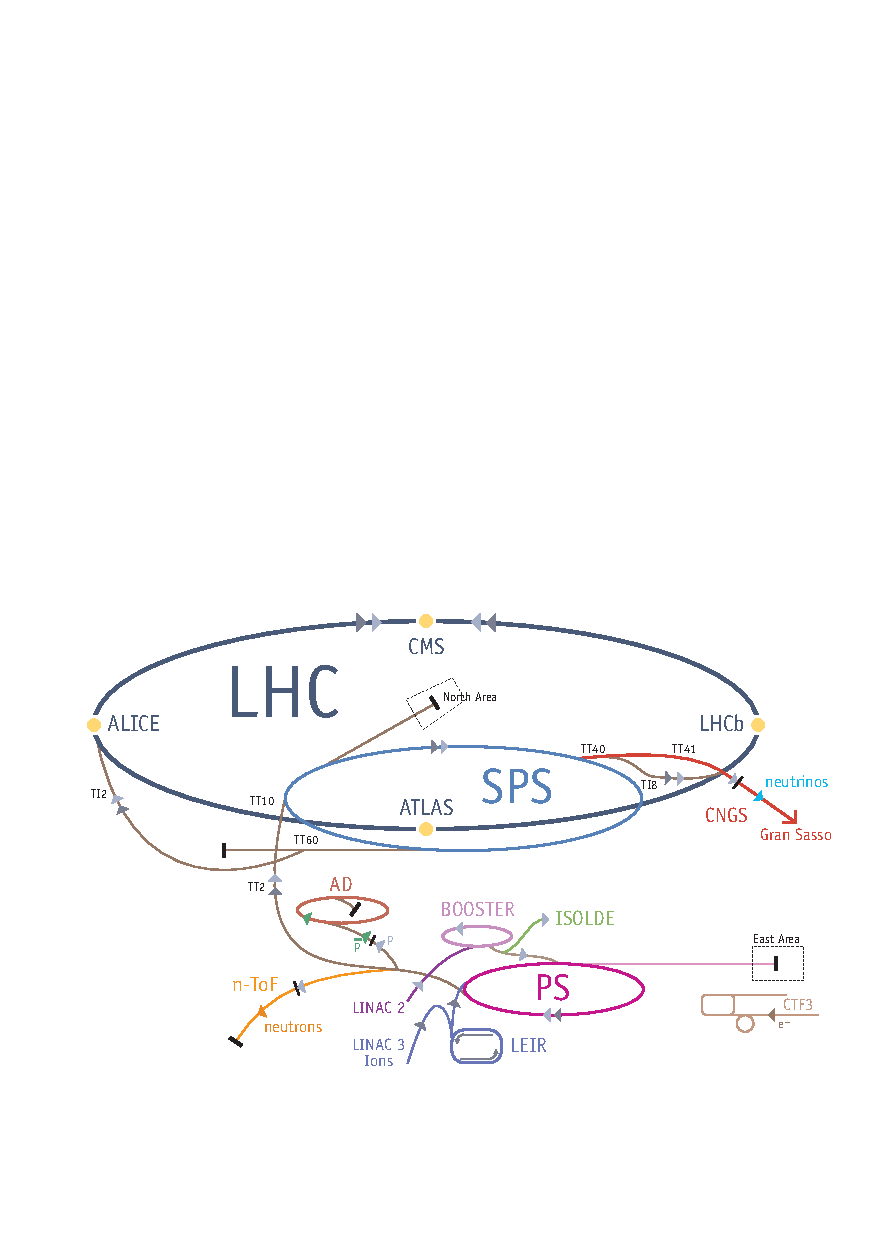
\includegraphics[width=0.90\textwidth]{fig/atlas/accel-chain.pdf}
  \caption{The LHC accelerator complex boosts particles to increasingly higher energies before reaching the LHC. The particle beams are accelerated successively by Linac 2, the Proton Synchrotron Booster (PSB), the Proton Synchrotron (PS), the Super Proton Synchrotron (SPS) and then finally enter the LHC rings~\cite{cern-faq}.}
  \label{fig:lhc-chain}
\end{figure}
\section{Beam conditions}
Due to the Radio Frequency (RF) fields in the accelerating cavities, the proton beams are segmented into groups of protons called \textit{bunches}. Each beam contains 2808 bunches, and each bunch contains 1.7$\times$10$^{11}$ protons. Many protons are included per bunch to maximize the probability of a proton-proton collision for a given bunch crossing. A bunch crossing occurred every 50 nanoseconds during operations in 2012.

Given two equally bunched beams, the \emph{instantaneous luminosity} ($\mathcal{L}$) is given by~\cite{PDG}:
\begin{equation}\label{eqn:lumi}
  \mathcal{L} = f \frac{n_1 n_2}{4\pi \sigma_x\sigma_y},
\end{equation}
where $f=\SI{11245.5}{\hertz}$ is the collision frequency of the LHC beams; $n_{1}$ and $n_{2}$ are the numbers of protons in each beam; and $\sigma_{x}$ and $\sigma_{y}$ are the RMS beam widths in the horizontal (bend) and vertical directions. The maximum instantaneous luminosity of the LHC in 2012 was 7.7$\times$10$^{33}$ cm$^{-2}$ s$^{-1}$.

The instantaneous luminosity must be integrated over time to obtain total luminosity. The beam conditions that go into Equation~\ref{eqn:lumi} change over the duration of a run. The integral over time and varied beam conditions is called the \emph{integrated luminosity} and can be used to relate the number of events $N$ for a given physics process to its cross section $\sigma$:
\begin{equation}\label{eqn:nevt}
  N = \sigma \times \int{\mathcal{L}(t) dt}
\end{equation}
In 2012, the total integrated luminosity of the LHC was 20.3 fb$^{-1}$ with uncertainty of 2.8\% \cite{Lumi}. The cumulative luminosity recorded over the course of 2012 is shown in Figure~\ref{fig:2012lumi}.
\begin{figure}[tp]
  \centering
  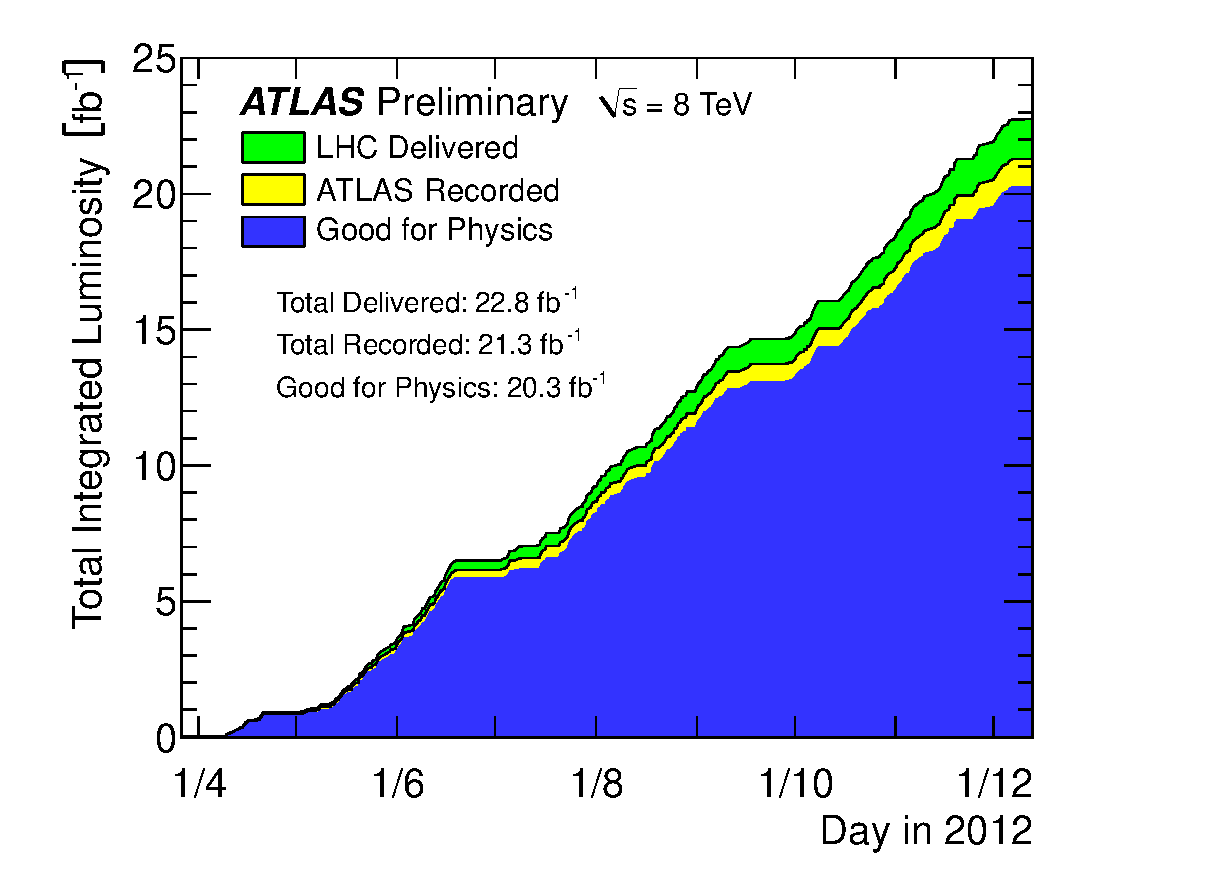
\includegraphics[width=0.90\textwidth]{fig/atlas/intlumivstime2012DQ.eps}
  \caption{Cumulative luminosity versus time delivered to (green), recorded by ATLAS (yellow), and certified to be good quality data (blue) during stable beams and for pp collisions at 8 TeV center-of-mass energy in 2012. Luminosity can be lost due to data acquisition inefficiency or other effects.}
  \label{fig:2012lumi}
\end{figure}

The beam conditions also determine the number of proton-proton interactions that occur in a single bunch crossing. When a single bunch crossing produces multiple separate proton-proton collisions, these events are referred to as \textit{pileup}. Pileup presents a significant challenge since it can rapidly increase the combinatoric complexity of reconstructing events and degrade the performance of the reconstruction algorithms. Figure~\ref{fig:atlas-pileup} shows the mean number of interactions per bunch crossing for 2011 and 2012, demonstrating the substantial increase of pileup events in the latter. Reconstruction challenges were overcome by optimizing the existing reconstruction algorithms, as well as new techniques for subtracting pileup events from the physics of interest~\cite{pileup}. 

\begin{figure}[tp]
  \centering
  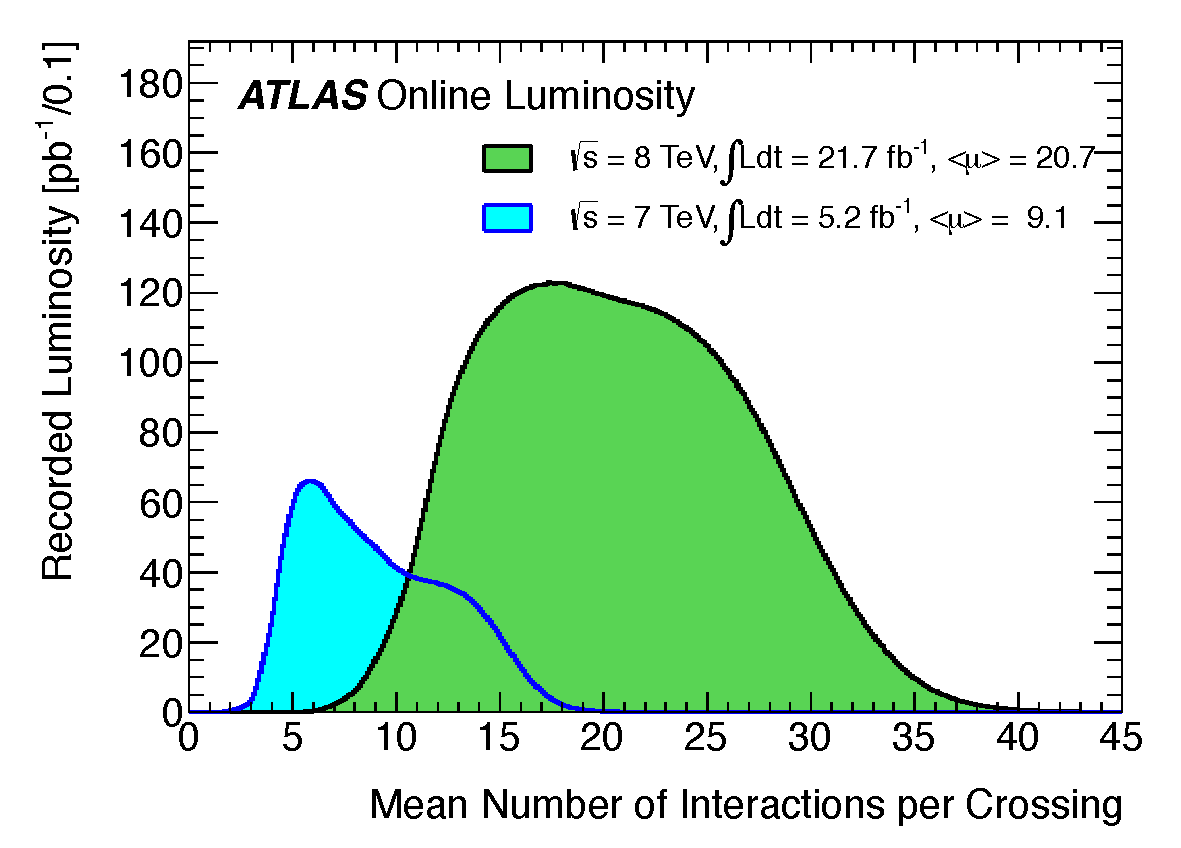
\includegraphics[width=0.90\textwidth]{fig/atlas/pileup.pdf}
  \caption{Luminosity-weight distribution of the mean number of interactions per bunch crossing. Both the full data from the 2011 and 2012 $pp$ runs at the LHC are shown.}
  \label{fig:atlas-pileup}
\end{figure}



\section{Overview of the ATLAS detector}
The ATLAS detector is a general purpose detector centered over one of the four interaction points of the LHC. The detector is cylindrical in shape with a diameter of 25 meters, a length of 46 meters, and a weight of 7,000 tons; it contains around 100 million electronic channels and around 3,000 km of cables. Assembling the detector at CERN took 5 years and was completed in 2008. A schematic rendering of the ATLAS detector is shown in Figure~\ref{fig:atlas-cgi}.
\begin{figure}[tp]
  \centering
  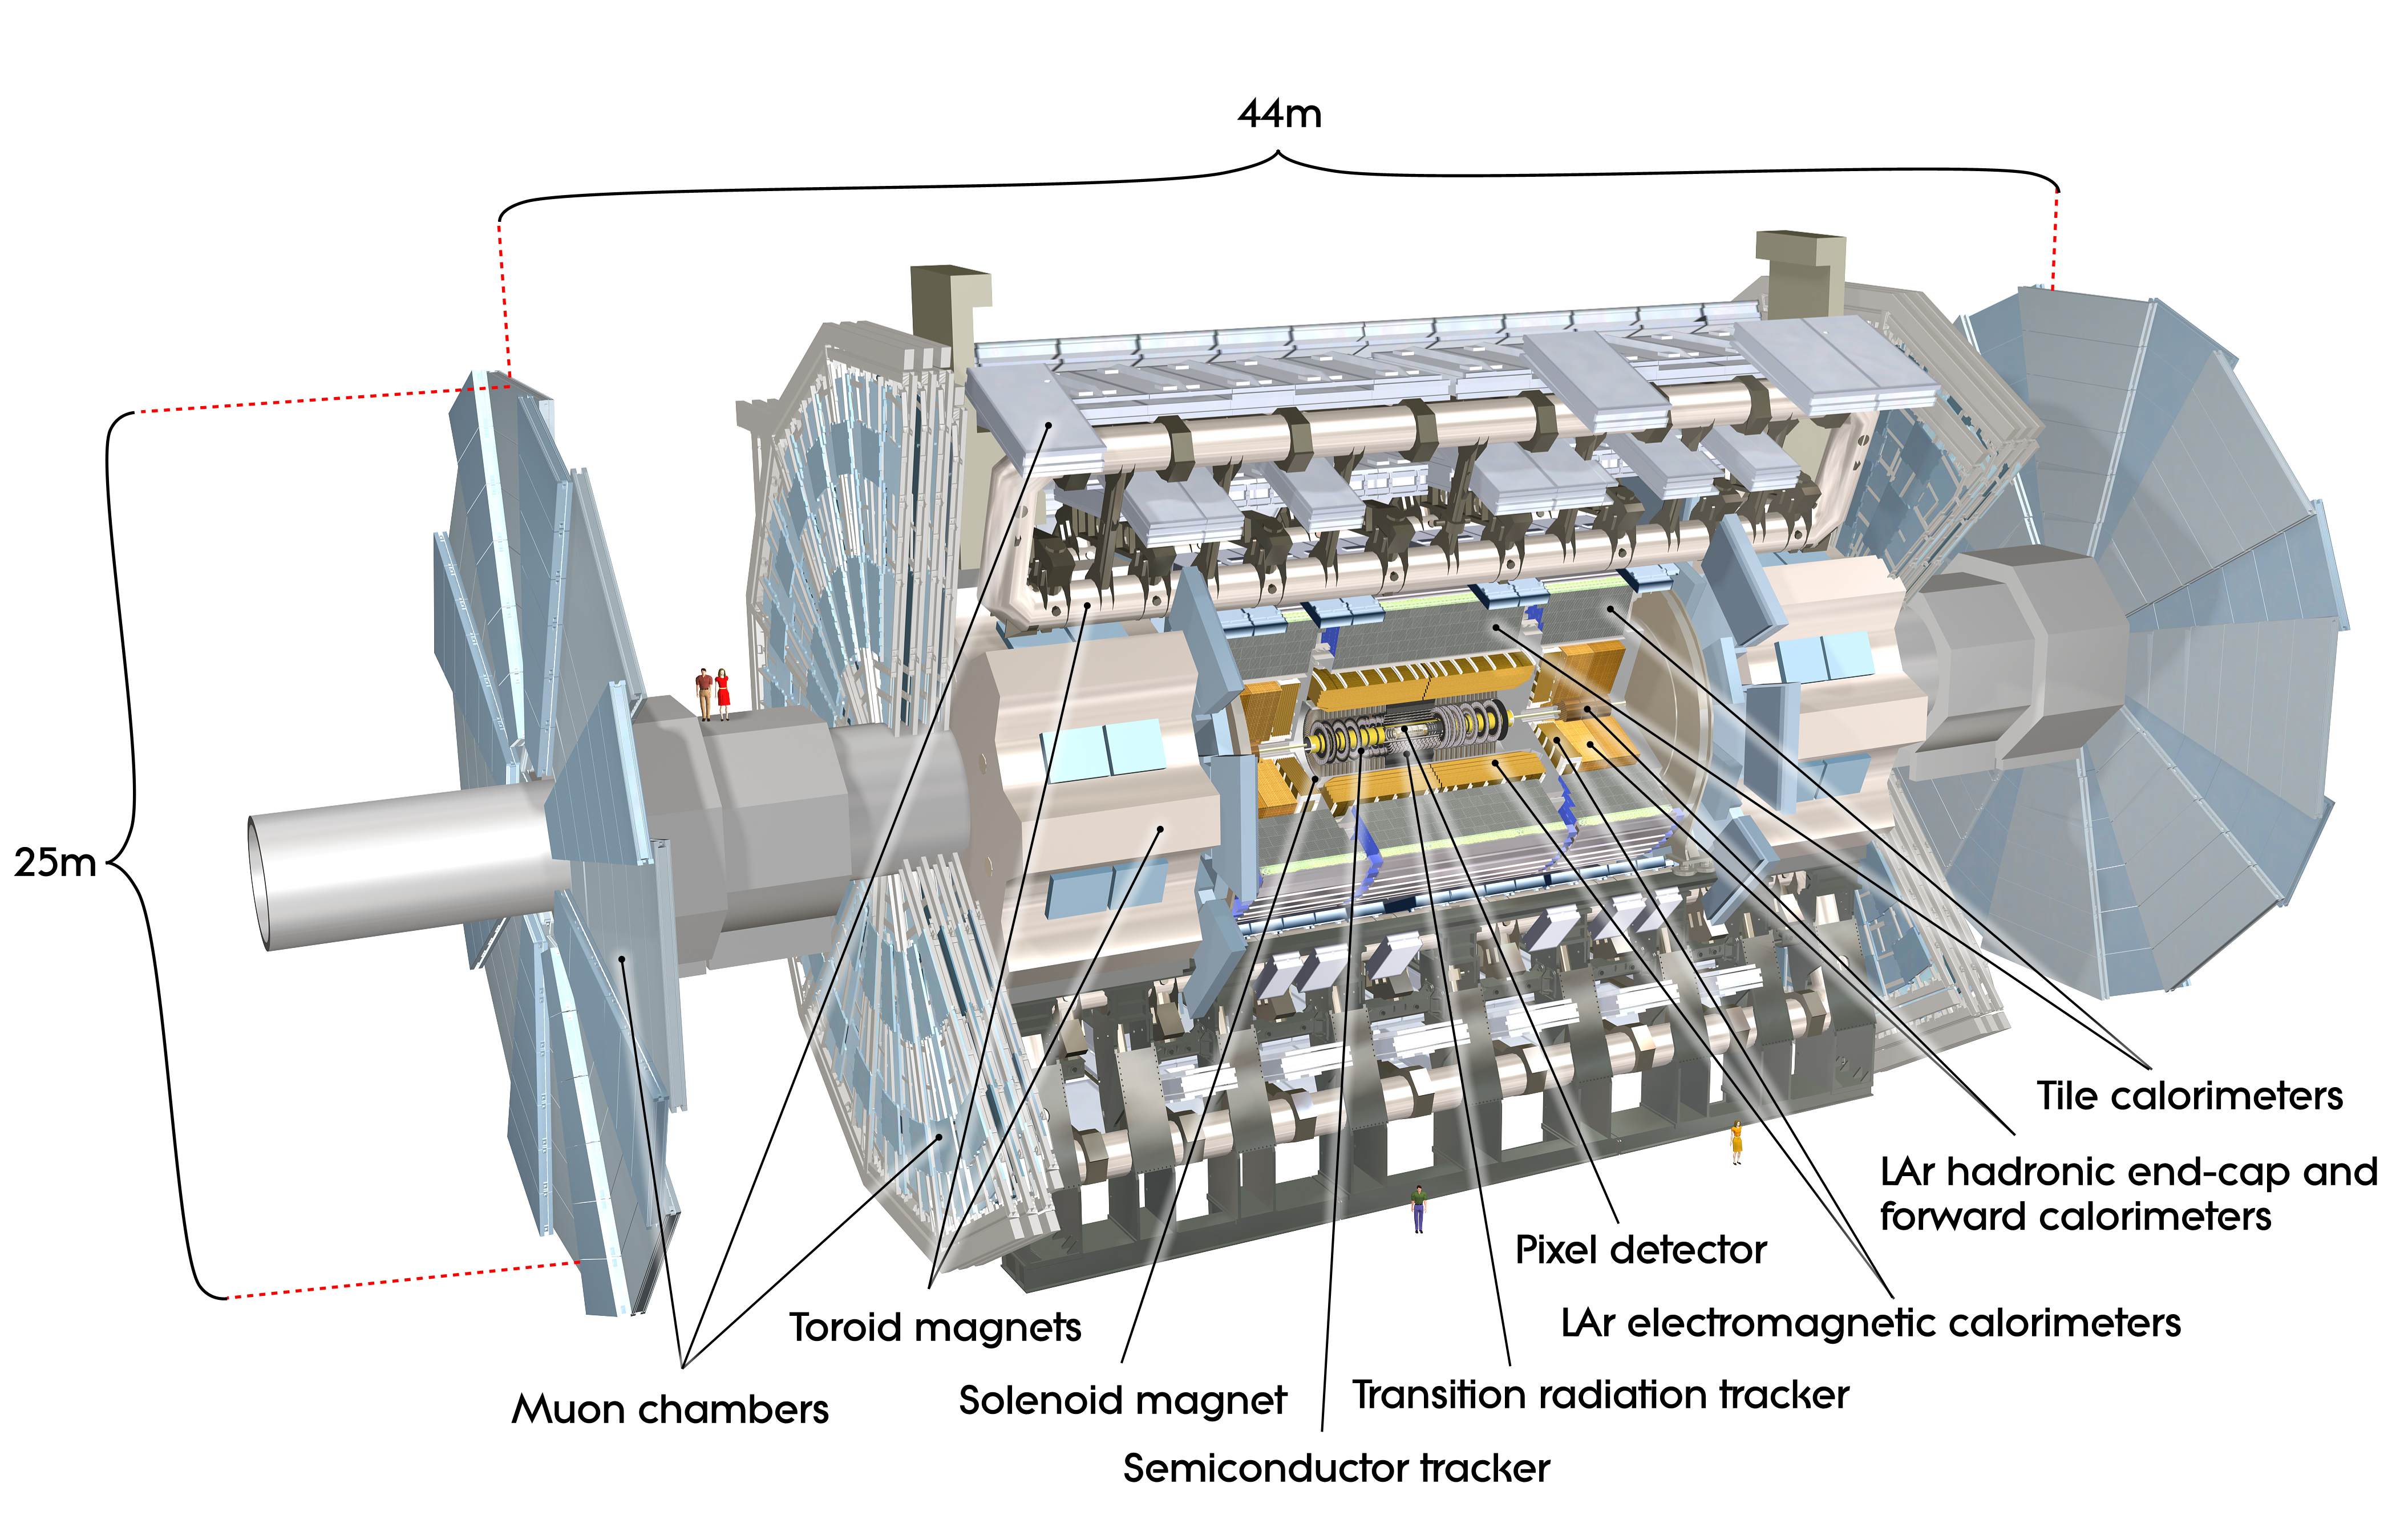
\includegraphics[width=0.90\textwidth]{fig/atlas/atlaspic.jpg}
  \caption{Computer generated illustration of the whole ATLAS detector detector, with various subdetectors highlighted\cite{Pequenao:1095924}.}
  \label{fig:atlas-cgi}
\end{figure}
In order to detect a wide range of physics processes in proton-proton collisions, ATLAS must measure the trajectory and energy of many different kinds of particles, including electrons, muons, photons, pions, kaons, protons and neutrons. Once these stable final-state particles are detected, information about the heavier, unstable particles can be inferred. This process is called \emph{reconstruction} and is discussed in detail in Chapter~\ref{ch:objects}.

ATLAS consists of specialized subdetectors designed to capture different phenomena. These subdetectors are arranged as increasingly larger concentric cylinders around the interaction point (IP) where the LHC proton beams collide. There are three main specialized sub-systems: the \emph{inner detector} (ID), which is located just outside the beamline and uses silicon and transition radiation systems to track the trajectory of charged particles; the \emph{calorimeters}, which are located radially outward from the ID and designed to measure the energy of particles with a shower sampling method; and the \emph{muon system}, which is located farthest from the IP and measures muon momentum and trajectory. Details of the subdetectors are provided below. An overview of interaction of different types of particles with the subdetectors as they travel through the detector is illustrated in Figure~\ref{fig:atlas-wedge}.
\begin{figure}[tp]
  \centering
  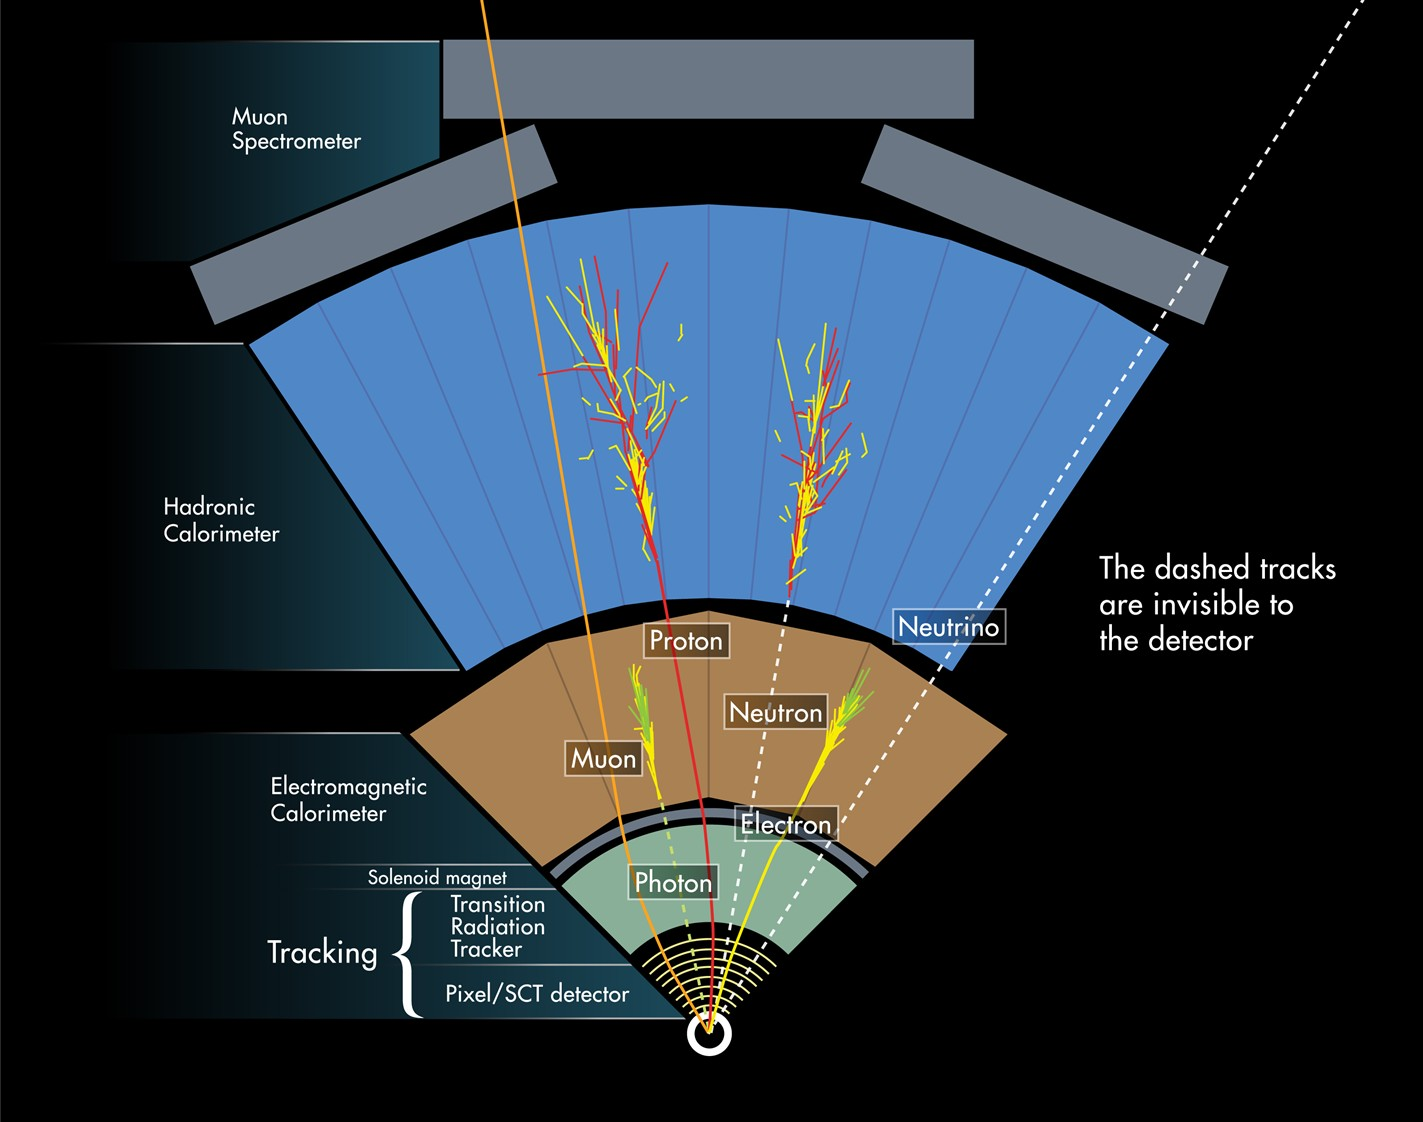
\includegraphics[width=0.90\textwidth]{fig/atlas/atlas-wedge.jpg}
  \caption{A computer-generated image representing how the ATLAS detector functions. The transverse paths of different types of particles are shown interacting with different elements of the detector\cite{atlas-wedge}.}
  \label{fig:atlas-wedge}
\end{figure}

ATLAS has a magnet system that bends the trajectory of charged particles as they travel through the detector. This allows the particles' momenta to be precisely calculated using the classical Lorentz force equation. The magnet system consists of a double configuration. Just outside the ID is a solenoid magnet that produces a field of approximately 2 Tesla. A large toroidal magnet within the outermost part of the detector produces a 1 to 2 Tesla field.


\subsection{Coordinate system}


ATLAS uses a right-handed coordinate system with its origin at the IP in the center of the detector, which is illustrated in Figure~\ref{fig:atlas-coord}. The $z$-axis along the beamline with the positive direction counter-clockwise around the LHC. The $x-y$ plane is defined such that the coordinate system is right-handed, with the $x$-axis pointing from the IP to the center of the LHC, and the $y$-axis pointing upwards. This plane is usually referred to as the transverse plane, since it is perpendicular to the beamline. Cylindrical coordinates, $r$ and $\phi$, are used in the transverse plane with $\phi$ defined as the azimuthal angle around the beamline. Instead of the polar angle from the beamline, $\theta$, pseudorapidity is typically used and is defined as:
\begin{equation}
\eta = -\text{ln}(\text{tan}\frac{\theta}{2})
\label{eq:eta}
\end{equation}
The pseudorapidity is used because in the limit of a massless particle, it is invariant with respect to Lorentz boosts along the beamline. The solid angle distances $\Delta R$ can be measured using the difference in pseudorapidity and azimuthal angle:
\begin{equation}
\Delta R = \sqrt{\Delta \phi^2 + \Delta \eta^2}
\label{eq:dR}
\end{equation}


\begin{figure}[tp]
  \centering
  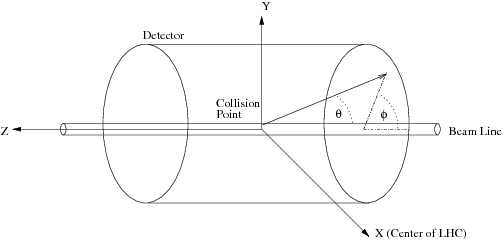
\includegraphics[width=0.90\textwidth]{fig/atlas/coord}
  \caption{Illustration of the ATLAS coordinate system\cite{Schott:2014sea}.}
  \label{fig:atlas-coord}
\end{figure}

% \subsection{Magnets}


%  The solenoid magnet is placed inside the electromagnetic (EM) calorimeter. This is different from most other detector designs where the magnet is placed outside the EM calorimeter. The advantage of the small solenoid is a compact design. A small magnetic field in the EM calorimeter also reduces the transverse spread of showers. The major problem is the increased amount of material in front of the calorimeter which causes many particles to start showering before they reach the active part of the calorimeter.
% The solenoid is a superconducting magnet kept at 4.5 K. To reduce the material the magnet does not have a separate cryostat but rather it shares the cryostat with the liquid argon calorimeter thus saving two cryostat walls. The half length of 2.65 m is considerably shorter than the inner tracking detector. This is a result of a compromise: a short coil reduces the material in front of the calorimeter; a long coil makes the magnetic field more uniform in the Inner Detector. The magnetic field along the z-direction drops from 2 T at the interaction point to around 0.5 T at the end of the Inner Detector.

% The toroid magnet system is divided into one barrel part and two forward systems. With a toroid field, particles will across the complete pseudorapidity range, be almost perpendicular to the field. This means that the field integral  $\int$Bdl , which is the important factor for momentum resolution, can be kept high even in the forward direction. The structure is open with 8 coils in the central region each in separate cryostats. One of the rectangular shaped cryostats can be seen in the front of fig. 4.1. In the forward direction the toroid field is also formed by 8 superconducting coils but there placed in a common cryostat.

% The low number of coils to form the toroid field results in a field strength that varies strongly with the  $\phi$ coordinate. The field integral varies in the barrel from 2-6 Tm and in the end-caps from 4-8 Tm. This is not ideal but an economical necessity.





\section{Inner detector}
The ID is a series of detectors that function as a tracking system to measure the momenta and trajectory of charged particles~\cite{cern-jinst-atlas}. This also allows reconstruction of the primary and secondary vertices of the collision. The innermost part of the entire detector is the pixel detector, 3 layers of silicon that accurately measure the three-dimensional spatial position of charged particles. Next is the SemiConductor Tracker (SCT), 4 layers of double-sided silicon strip modules which accurately measure tracks in the $r-\phi$ plane and are double sided to provide stereo information along the $z$ axis. The outermost component of the ID is the Transition Radiation Tracker (TRT), straw tubes filled with Xenon gas interleaved with polymer layers which provides additional trajectory measurement and differentiate between electron and hadrons. Figure~\ref{fig:id-scheme} shows a schematic outline of the entire inner detector, and Figure~\ref{fig:id-barrel} illustrates a cut-away view of the inner detector barrel.

\begin{figure}[tp]
  \centering
  \includegraphics[width=0.7\textwidth]{fig/atlas/id-schem}
  \caption{Schematic view of the Inner Detector: an $r-z$ slice of the cylindrical barrel, disc endcaps with support tubes, and the solenoid magnet. Lines of constant $\eta$ are drawn~\cite{cern-jinst-atlas}.}
  \label{fig:id-scheme}
\end{figure}
\begin{figure}[tp]
  \centering
  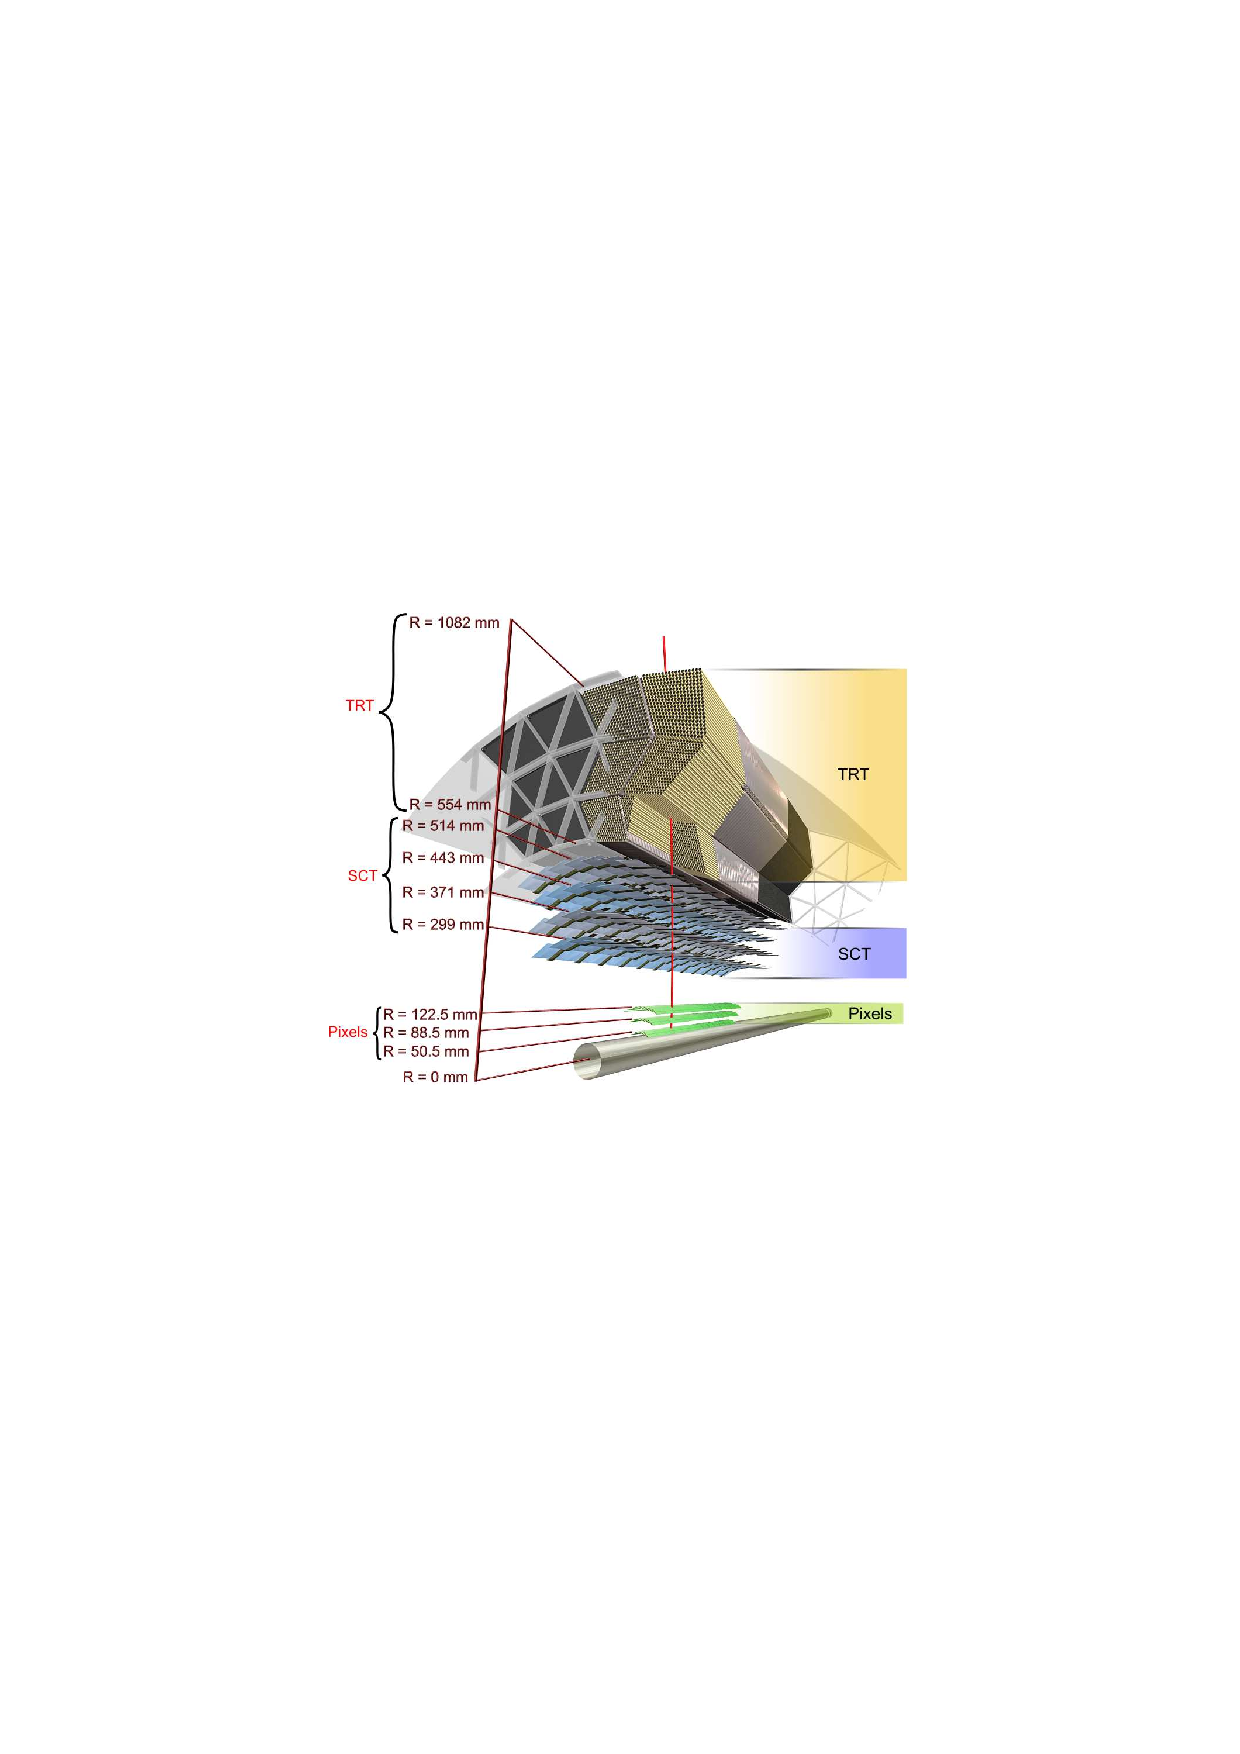
\includegraphics[width=0.7\textwidth]{fig/atlas/id-barrel}
  \caption{A diagram of the barrel of the Inner Detector: the three layers in the Pixels, the four layers in the SCT, and the many layers of the TRT~\cite{cern-jinst-atlas}.}
  \label{fig:id-barrel}
\end{figure}
\subsection{Pixel detector}
The pixel detector is located closest to the beamline and is designed to provide fine granularity in a high radiation environment. Measuring trajectories closest to the interaction point is important for constructing the secondary vertex, necessary for the $b$-tagging of jets used in this analysis.

The pixel detector has 3 barrel layers and three endcap disks on each side of the barrel. The barrel layers are located 50.5 mm, 88.5 mm and 122.5 mm radially from the interaction point. The endcaps sit at 495 mm, 580 mm and 650 mm away from the interaction point. Together, they provide coverage up to $|\eta|=2.5$.

Each silicon pixel in these layers is a p-n junction built of n-type bulk with both p$^+$ and n$^+$ impurities. The additional n$^+$ implants allow the pixels to operate even after the inversion of the bulk from n-type to p-type caused by the high radiation dose. The size of each pixel is $50 \times 400 \micron^2$ with the longer side along the $z$ direction. This allows charged particle hit resolution of approximately 115 $\mu$m in the direction of the $z$ axis and 10$\mu$m in the direction of the transverse plane.

Pixels are bump-bonded to front-end readout chips, with a grid of 2880 pixels connected to each chip. Front-end chips are grouped into rectangular \emph{modules} of dimension $19 \times 63 \micron^2$. Modules in the barrel layers are arranged into long structures parallel to the beamline called \emph{staves}. Staves are tiled at $20^{\circ}$ with respect to the radial direction and overlapped to provide full azimuthal coverage. Endcap modules are arranged into petals and then into wheels, with the sensing element perpendicular to the beam axis. These supporting structures also host power, clock, command and data lines to and from each module. Full coverage is ensured in the endcaps by alternating the placement of the sensors on the front and back of the wheel. The arrangement of the barrel and endcap layers ensures that charged particles with $|\eta|<2.5$ will pass through at least three pixels.

\subsection{SemiConductor Tracker}
The SCT surrounds the Pixel detector and also employs silicon detector elements, using micro-strips instead of pixels. The strips are arranged in four double layers, with the pairs arranged at small angles relative to each other, to make a three-dimensional measurement. The SCT has 4 barrel layers and 2 endcaps, each with 9 disks. 

The SCT is made of single-sided p-in-n sensors of thickness $285\ \micron$ with readout strips. In the rectangular barrel sensors, the readout channels are arrange with a pitch of $80\ \micron$ between them, and the trapezoidal endcap sensors have radial strips with a mean pitch of  $80\ \micron$.  Modules are comprised of four sensors arranged in two layers aligned at a stereo angle of 40 mrad with respect to each other. This allows a single module to measure all three dimensions spatial position of a charged particle passing through both the front and back layers. The endcap wheels are arranged so that charged particles with $|\eta|<2.5$ will pass through at least eight sensors. The 2112 modules in the barrel have resolution a $17\ \micron$ of in $r-\phi$ and $580\ \micron$ in $z$, and the 1976 endcap modules have a resolution of $17\ \micron$ in $r-\phi$ and $580\ \micron$ in $r$.

\subsection{Transition Radiation Tracker}
The outermost layer of the ID is the Transition Radiation Tracker (TRT). The TRT extends the tracking volume to 1106 mm and also distinguishes between electrons and pions based on their transition radiation as they pass through. It consists of straw drift tubes 4 mm in diameter filled with a Xenon gas mixture. At the center of each tube is a 35 $\micron$ diameter anode tungsten wire held at ground potential. Charged particles ionize the gas inside the tube, then the electric field between the tube and the wire creates an ionization cascade, which can be used to infer the energy of the original particle.

The 351,000 tubes are arranged in a barrel and two endcaps. In the barrel, 73 layers of 144 cm long tubes are parallel to the beamline, with wires slit in half to allow separate measurements for positive and negative $z$. In the endcaps, the 160 layers of 37 cm long tubes are arranged radially.  The intrinsic resolution of the TRT in the barrel is $130\ \micron$ in $r\phi$ with coverage up to $|\eta|<2.0$. A charged particle usually passes through 30 or more tubes.

When charged particles pass through a polymer fiber mat sitting between the tubes, transition radiation may be produced. These photons from transition radiation produce an ionization cascade much higher than the signal for tracking minimum-ionizing particles. Therefore, TRT straws have two signal thresholds: a \emph{high threshold} for transition radiation hits and a \emph{low threshold} for tracking hits. 

Transition radiation, produced when a charged particle crosses the boundary between two media of different dielectric constants, is proportional to the Lorentz $\gamma$ of a particle. For an electron and charged pion of equal momentum, the electron is about 3.7 times more likely to produce transition radiation than the pion since its mass is 200 times smaller. Seven to ten high threshold hits are typical when an electron passes through the TRT. 



\section{Calorimeters}
The calorimeter system  stops and measures the energy of electrons, photons and jets with full coverage in $\phi$ and $|\eta|<4.9$. This is done with separate electromagnetic and hadronic calorimeters, both with barrel and endcap components. A forward calorimeter provides high $\eta$ measurements. ATLAS calorimeters are sampling calorimeters, which means that only part of the shower energy is observed. Absorbing material used to initiate showers is interleaved with active material for detecting the showers. The layout of the calorimeters can be seen in Figure~\ref{fig:calo}. 

\begin{figure}[tp]
  \centering
  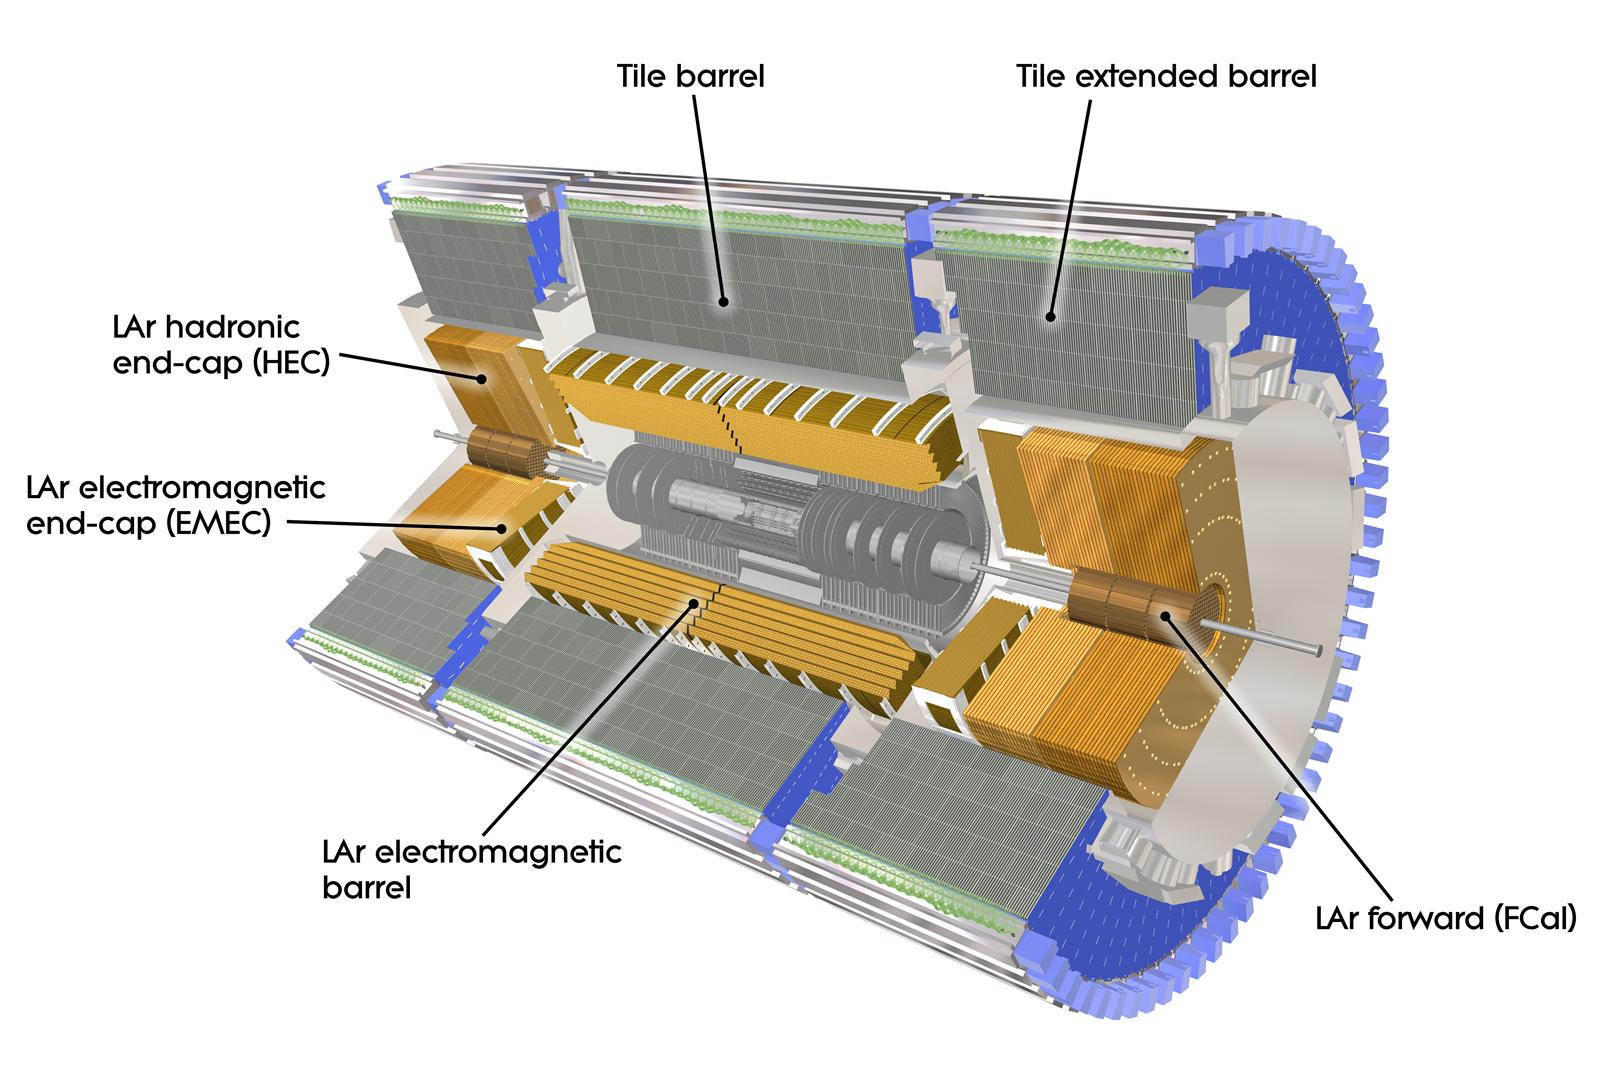
\includegraphics[width=0.95\textwidth]{fig/atlas/combinedCalo}
  \caption{Cut-away view of the ATLAS calorimeter system~\cite{cern-jinst-atlas}.}
  \label{fig:calo}
\end{figure}
\subsection{Electromagnetic calorimeter}
The EM calorimeter has alternating lead absorbers and liquid argon (LAr) active medium with kapton electrodes. The barrel component covers $|\eta| < 1.5$ and the endcap component cover $1.4 < |\eta| < 3.2$. A presampler layer covering $|\eta| < 1.8$ measures showers starting before the calorimeter. 

The barrel is segmented into three layers of decreasing segmentation. The first and second layers are important for identifying shower shapes, so they are finely segmented. The first layer has a thickness of 4.3 $X_0$, and the second layer has a depth of 16 $X_0$, which usually contains the majority of the energy of the EM shower. The third layer is a shallow 2 $X_0$ to capture any leftover energy after the first two layers. To provide prevent gaps in $\phi$, the layers are bent into an accordion-like shape. A diagram of a barrel module is shown in Figure~\ref{fig:caloModule}. The endcap of the EM calorimeter goes out to $|\eta|<$ 3.2 and also has two layers, with an accordion shape oriented such that gaps in $\eta$ are prevented.




\begin{figure}[h]
\begin{minipage}[b]{0.48\textwidth}
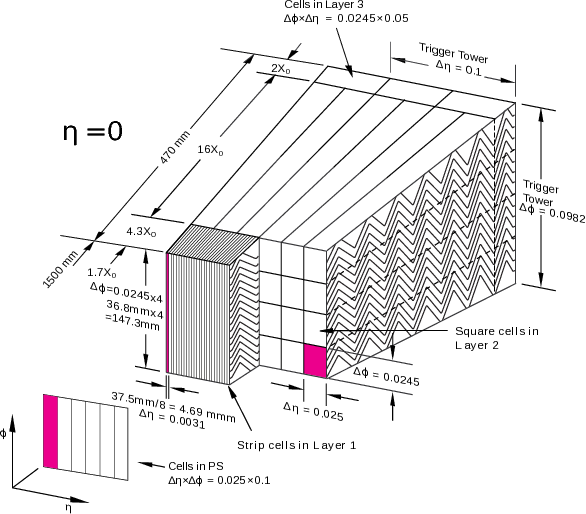
\includegraphics[width=\textwidth]{fig/atlas/caloModule.png}
\caption{Diagram of an electromagnetic calorimeter barrel module\cite{cern-jinst-atlas}.}
\label{fig:caloModule}
\end{minipage}
\hfill
\begin{minipage}[b]{0.48\textwidth}
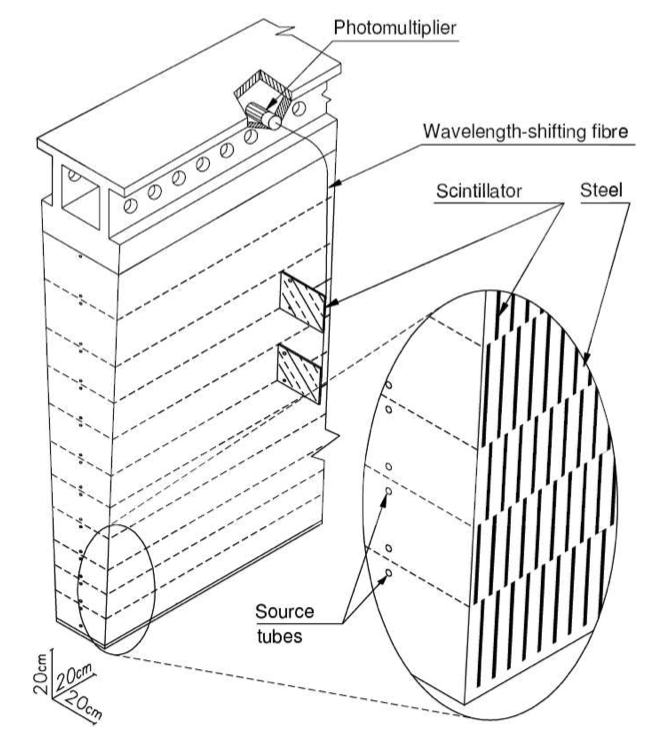
\includegraphics[width=\textwidth]{fig/atlas/tile.png}
\caption{Diagram of a hadronic tile module\cite{cern-jinst-atlas}.}
\label{fig:tileModule}
\end{minipage}
\end{figure}
\subsection{Hadronic calorimeter}
The hadronic calorimeter is divided into three components: the barrel tile calorimeter, which uses steel absorbers and scintillator tiles and covers $|\eta| <$1.7; the Hadronic Endcap Calorimeter (HEC), which uses copper absorber and LAr active material and covers $|\eta|$<3.2; and the forward calorimeter (FCal), which uses LAr active materials and covers $3.1 < |\eta| < 4.9$. The hadronic calorimeters are much coarser than the EM calorimeters because electrons and photons usually don't reach the radius of the hadronic calorimeters, so particle identification isn't a priority. Figure~\ref{fig:tileModule} shows a schematic of a hadronic tile module.
\subsection{Clustering}
\label{ss:cluster}
In order to identify particles, information from the shape of the calorimeter showers must be used. EM particles like photons and electrons produce narrow showers which are largely contained in the EM calorimeters. Hadrons produce broader showers and tend to travel farther into the hadronic calorimeters. Hadronic showers can also contain EM deposits from decays before the calorimeters, such as a neutral pion becoming two photons. In order to turn energy deposits in cells into clusters, information from all of the calorimeters is used as inputs to one of two principal algorithms\cite{ATL-LARG-PUB-2008-002}. The \emph{sliding-window} algorithm clusters cells within fixed-sized rectangles. This algorithm is generally used for electron, photon and tau identification. 

The second algorithm is the \emph{topological} algorithm, which clusters together neighboring cells on the condition that the energy deposit in the cell is significantly more than the expected noise. This algorithm is generally used for jet and missing transverse energy reconstruction. The clusters that result from this algorithm are called \emph{topoclusters.}


\section{Muon System}
The Muon System (MS) is the outermost subdetector, since muons are the only charged particles that can pass though the calorimeters~\cite{2010.muonspectrometer}. The MS consists of a toroidal magnet system and a charged particle tracking system. The components of the muon system, highlighted in Figure~\ref{fig:muonOverview}, are designed to measure the path and energy of muons, particularly high \pt\ muons which may indicate the presence of interesting physics.

The magnetic field provides the bending necessary for charge and momentum measurements and is comprised of three large air-core toroids. The toroid system has eight coils symmetrically around the beam and provides a magnetic field between 2 and 8 Tesla. 

There are two types of tracking systems in the MS. The Monitored Drift Tubes (MDTs) precisely measure the track in the bending direction of the magnetic field and cover $|\eta|<2.7$ in the outer barrel and cover $|\eta|<2.0$ in the inner barrel.  The MDTs are pressurized aluminum drift tubes filled with a mixture of argon and carbon dioxide gas, 30 mm in diameter. Each chamber has 3-8 layer of tubes and a resolution of 35 $\mu$m per chamber. The MDTs are limited to a counting rate of 150 Hz/cm$^2$ and thus cannot be used in the forward region of the inner layer, where high muon rates are expected. This region instead uses Cathode Strip Chambers (CSCs) for momentum measurement with better timing and spatial resolution. The CSCs cover the forward region of the inner layer, 2.0$<|\eta|<$2.7. Two endcap wheels each have 16 chambers. Each chamber has 4 CSC planes. Each plane consists of two cathode strip planes sandwiching anodes wire. The arrangement of the CSCs gives resolution of 40 $\mu$m radial direction and 7 ns timing resolution.

The MS also has two types of trigger chambers: Resistive Plate Chambers (RPC) in the barrel and Thin Gap Chambers (TGC) in the endcaps. Just as with tracking, the endcap and barrel have different types of triggers due to the different rate and precision requirements. The barrel trigger system has 3 RPC layers, and the endcap trigger system has 4 TGC layers. 

\begin{figure}[tp]
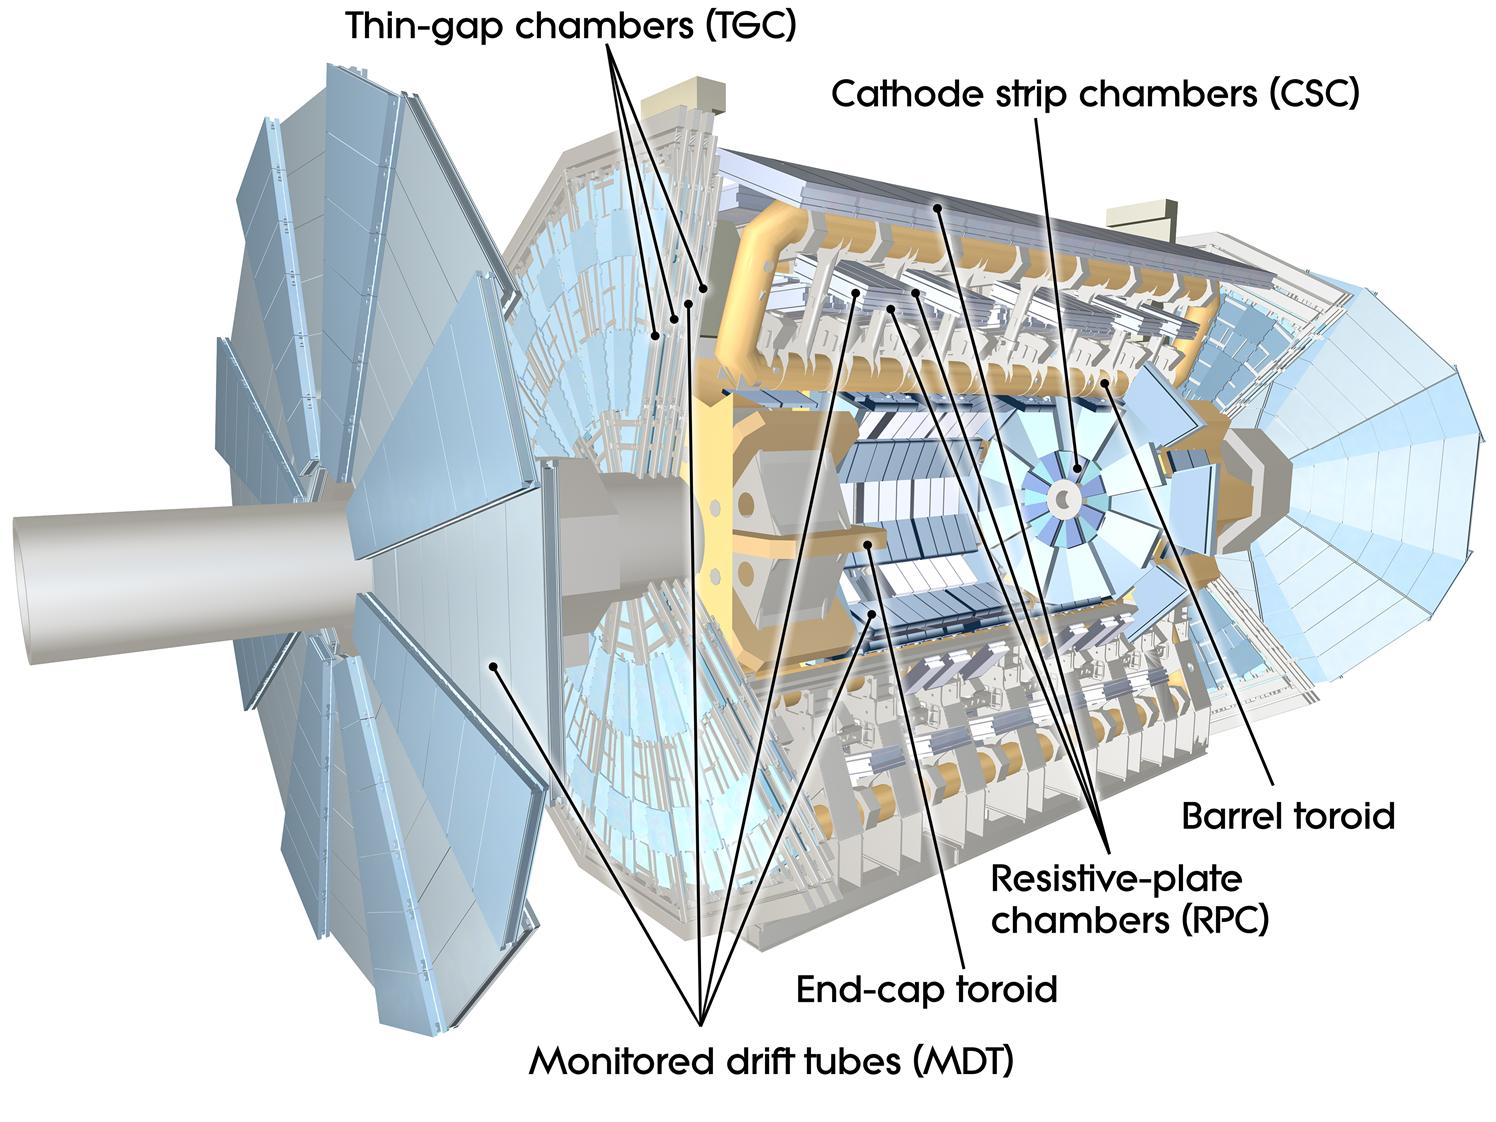
\includegraphics[width=0.95\textwidth]{fig/atlas/muonchamb.jpg}
\caption{Diagram of the muon system\cite{cern-jinst-atlas}.}
\label{fig:muonOverview}
\end{figure}


\section{The trigger system}
At hadron colliders, only a very small fraction of the proton-proton collisions can be feasibly recorded. The majority of events are low energy jets events that can be used for new physics searches or precision measurements like the Higgs are rarer. With bunch crossings every 50 ns, recording and reconstructing all of the collisions would take an unreasonable amount of data storage and computing power. It would also be impossible to write out events at this rate. Therefore, it is necessary to determine whether a collision will be recorded immediately after it occurs with minimal analysis. 

The process quickly filtering events to record only those of physics interest is called \emph{triggering.} Processes which take place in the trigger system are referred to as \emph{online}. Processes which take place after triggering, such as particle reconstruction, are called \emph{offline}.

The ATLAS trigger scheme\cite{TDR-L1} consists of three stages: Level 1 (L1), Level 2 (L2), and Event Filter (EF). All collision candidates are first run through L1, an online hardware trigger that has coarse granularity by necessity. If events pass the L1 trigger, they are then passed through the offline software triggers, collectively called the High Level Trigger (HLT) and divided into two stages: L2 and EF.

Applying multiplicity and energy threshold requirements, L1 reduces the rate of events from 20 MHz (all $pp$ collisions) to 75 kHz. The L1 trigger only looks at output from the calorimeters and muon system because the inner detector cannot process events at the rate required. In order to process events with the necessary speed, granularity in the calorimeter must be reduced and in the muon system, only the trigger chambers are read out. This reduction in granularity is illustrated in Figure~\ref{fig:l1}. The maximum latency time to process at this level is 2.5 $\mu$s. The data-acquisition system must keep track of which data correspond to which bunch crossing. This presents a substantial challenge since the time for measuring a signal shape in the EM calorimeter is $>100$ ns and the time of flight through the MS is $>25$ ns, both longer than the time between events. 

If the event passes the L1 trigger, then the L2 trigger looks at the distribution of energy deposits as Regions Of Interest (ROIs) identified by L1. The detector signals are compared to a menu of pre-programmed signatures that represent a potential physics object. For instance, a track and a cluster in the EM calorimeter might signal an electron. The L2 looks for these signatures in the ROIs by pulling information from all needed detectors. 

For events with signatures that pass the L2 trigger, all information for the event is read out and the standard offline reconstruction algorithm is run. The event can then be evaluated in terms of the fully reconstructed physics objects to see if particle identities and kinmatics match a menu of desired signatures. Finally, a decision about whether to record the event or not is made. This last stage of the triggering is called the Event Filter. The EF takes about 4s to process each event and can accept events at a rate up to 200 Hz.


\begin{figure}[tp]
  \centering
  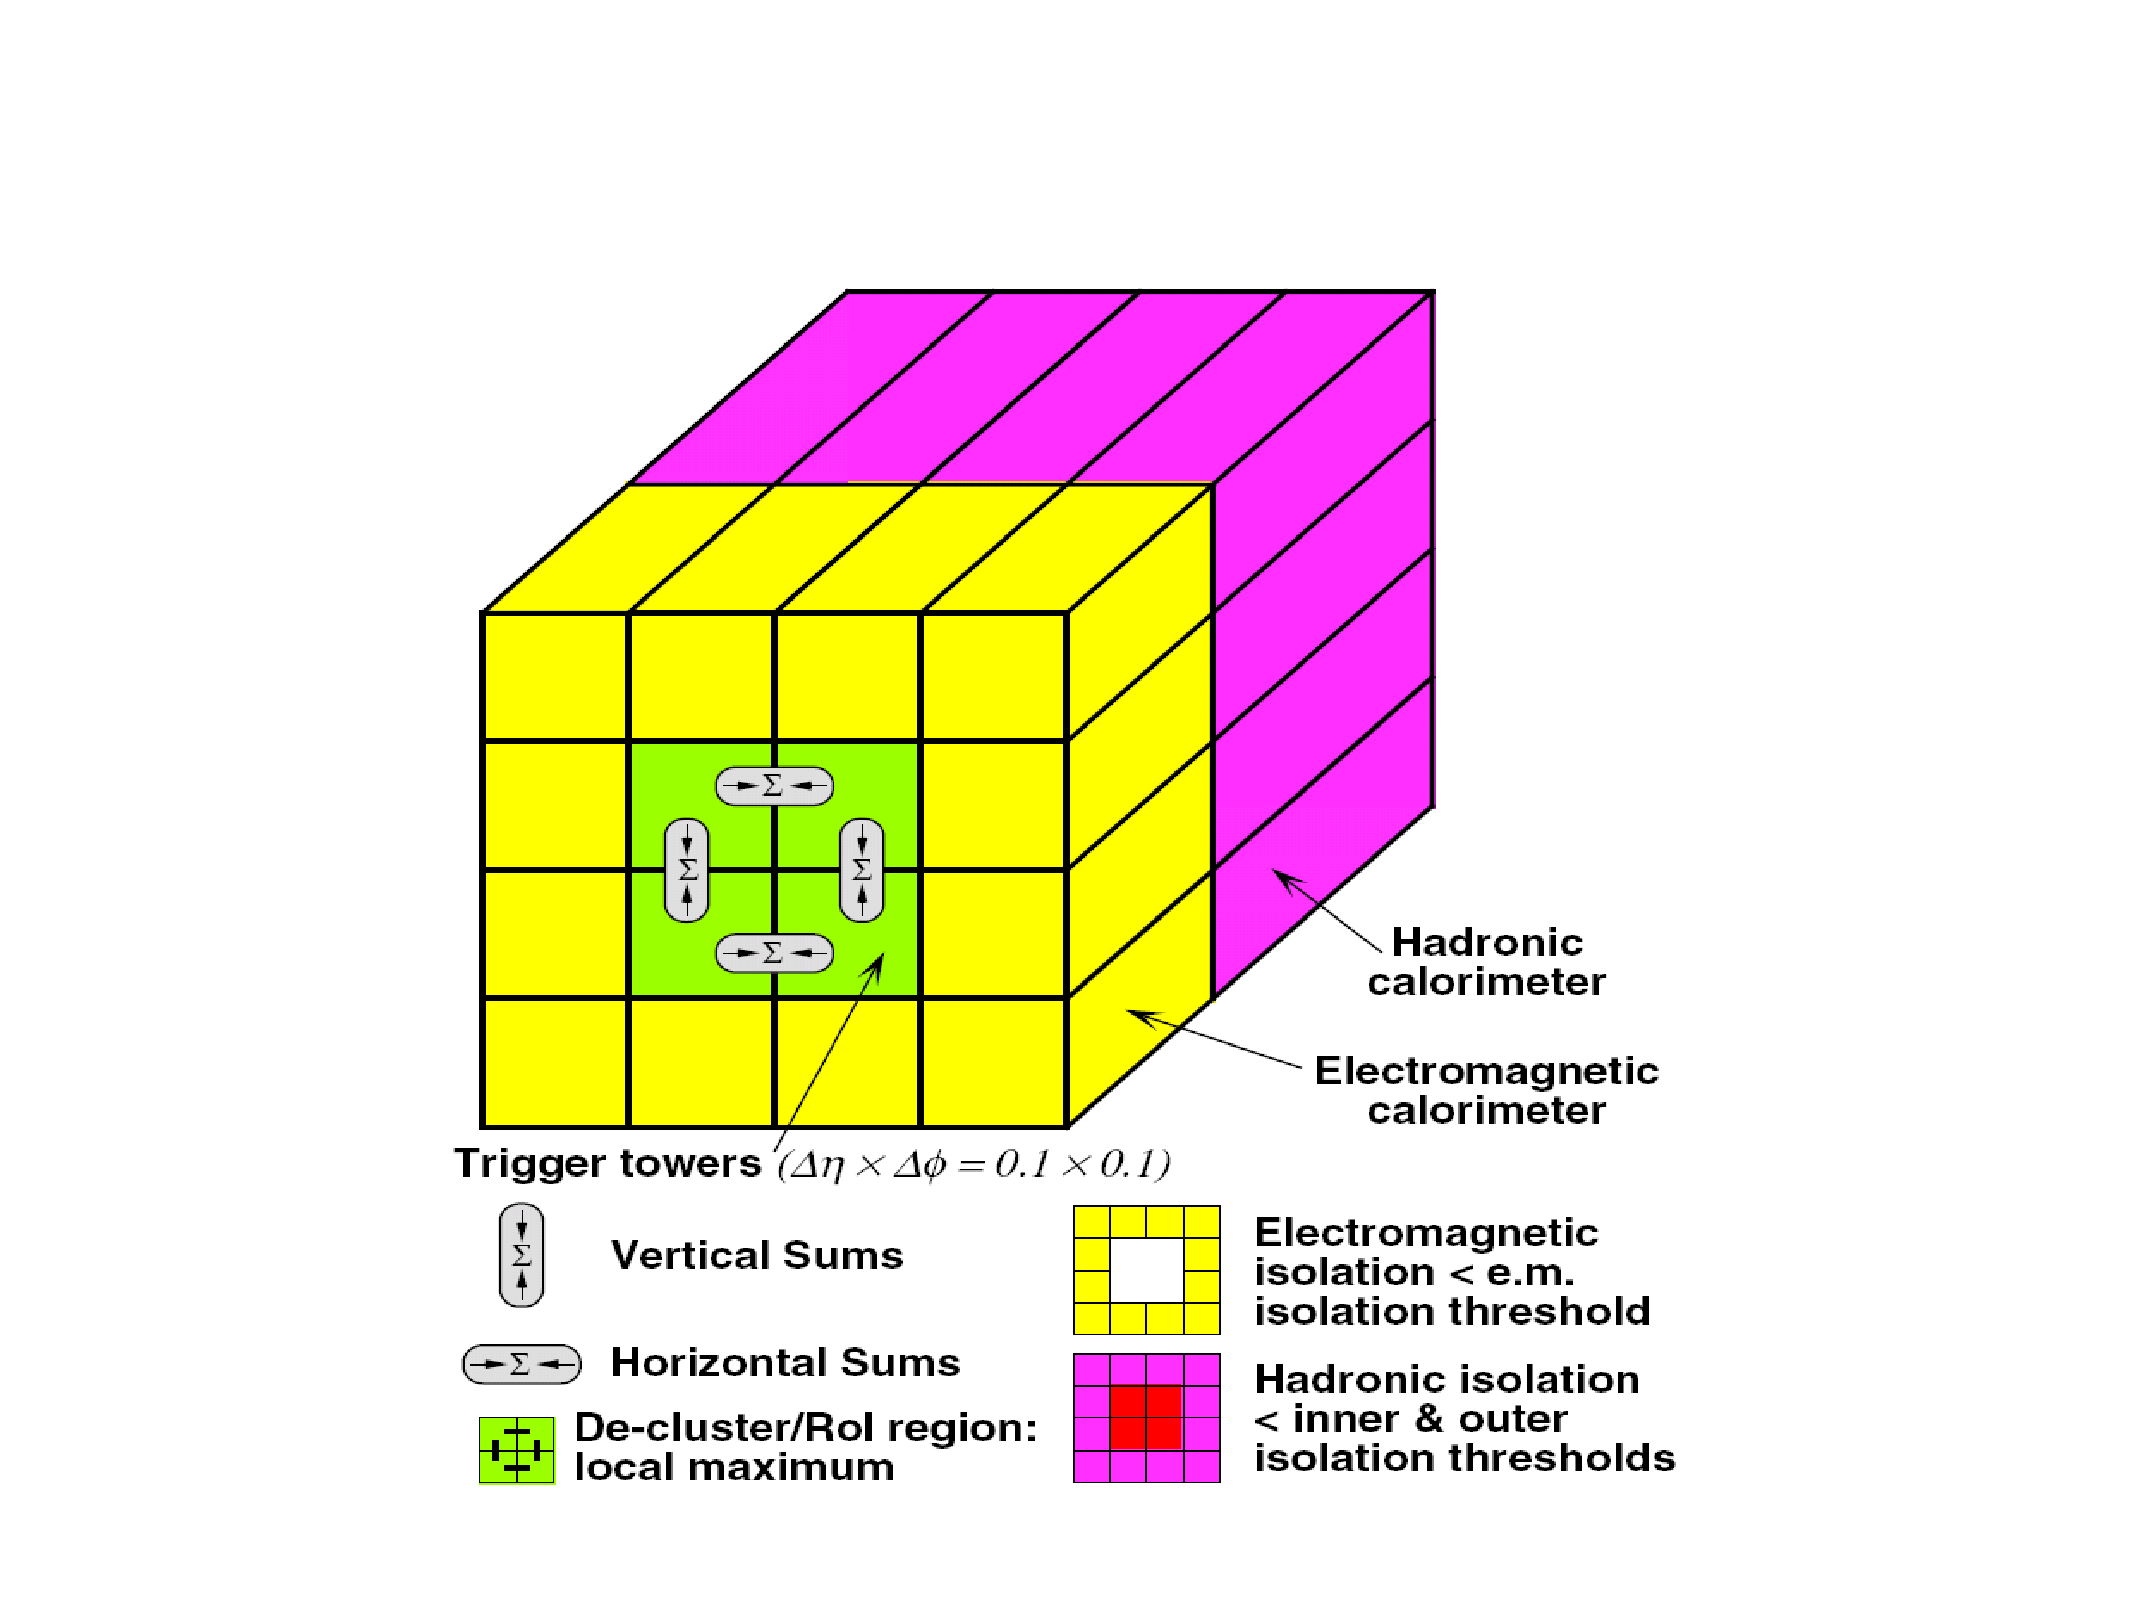
\includegraphics[width=0.80\textwidth]{fig/atlas/cartoonL1.pdf}
  \caption{Schematic view of the calorimeter granularity available at the L1 trigger~\cite{TDR-L1}.}
  \label{fig:l1}
\end{figure}
\subsection{Single electron trigger}
The single electron trigger used for 2012 is fully described in~\cite{eltrig}. At L1, calorimeters are split into $0.1\times0.1$ towers and then $2\times 2$ clusters are used to identify $e/\gamma$ leptons with the sliding window algorithm described in Section~\ref{ss:cluster}. Regions of $4\times 4$ with clusters that meet isolation requirements are passed to the L2 trigger as ROIs. At L2, the position of the cluster is identified as the energy-weighted average of the cluster. Track reconstruction is then performed and if a track can be matched to the cluster, it is considered to come from an electron, not a photon. At both L2 and EF, electron candidates are require to pass selection criteria based on the calorimeter cluster and the track, such as cuts on the lateral width of the shower and hits in the inner pixel detector.

In this analysis, the logical OR of two triggers is used to identify electrons: a 24 GeV trigger with a loose track-based isolation requirement and a 60 GeV trigger without an isolation requirement. The isolation requirement specifies that the sum of the \pt of tracks within a cone of $\Delta R$=0.2 must be less than 10\% the \pt of the electron. These trigger chains have thresholds that are maximally efficient for leptons passing offlines selections of $\pT > 25 \GeV$.

\subsection{Single muon trigger}

The single muon trigger used for 2012 is fully described in~\cite{mutrig}. The muon trigger uses data from the RPCs in the barrel region and the TGCs in the outer region. At L1, the paths between hits in the trigger chambers are interpolated to identify muon candidates. If a hit pattern matches the requirements of the L1 trigger, the $\eta$ and $\phi$ coordinates are passed to the L2 trigger as a ROI. At L2, the MDT and CSC information for the ROI are used to fit a higher quality track. Then, the track in the MS is combined with a track from the ID. Calorimeter data can be used to apply isolation requirements. Quality cuts are applied to the track to determine whether it passes the final trigger chain.

In this analysis, the logical OR of two triggers is used to identify muons: a 24 GeV trigger with a loose track-based isolation requirement and a 36 GeV trigger without an isolation requiment. The isolation requirement specifies that the sum of the \pt of tracks within a cone of $\Delta R$=0.2 must be less than 12\% the \pt of the muon. These trigger chains have thresholds that are maximally efficient for leptons passing offlines selections of $\pT > 25 \GeV$.

